% BEGIN
% ETH STYLE -> DON'T CHANGE
\documentclass[british,11pt,a4paper]{memoir}
\usepackage[utf8]{inputenc}
\usepackage[OT1]{fontenc}
\usepackage{babel}
\usepackage[sc]{mathpazo}
\usepackage{amsmath,amssymb,amsfonts,mathrsfs}
\usepackage[amsmath,thmmarks]{ntheorem}
% =======================================================
\usepackage{soul}
\usepackage{pdfpages}
\graphicspath{ {Pics/} }
%% See the TeXed file for more explanations

%% [OPT] Multi-rowed cells in tabulars
%\usepackage{multirow}

%% [REC] Intelligent cross reference package. This allows for nice
%% combined references that include the reference and a hint to where
%% to look for it.
\usepackage{varioref}

%% [OPT] Easily changeable quotes with \enquote{Text}
%\usepackage[german=swiss]{csquotes}

%% [REC] Format dates and time depending on locale
\usepackage{datetime}

%% [OPT] Provides a \cancel{} command to stroke through mathematics.
%\usepackage{cancel}

%% [NEED] This allows for additional typesetting tools in mathmode.
%% See its excellent documentation.
\usepackage{mathtools}

%% [ADV] Conditional commands
%\usepackage{ifthen}

%% [OPT] Manual large braces or other delimiters.
%\usepackage{bigdelim, bigstrut}

%% [REC] Alternate vector arrows. Use the command \vv{} to get scaled
%% vector arrows.
\usepackage[h]{esvect}

%% [NEED] Some extensions to tabulars and array environments.
\usepackage{array}

%% [OPT] Postscript support via pstricks graphics package. Very
%% diverse applications.
%\usepackage{pstricks,pst-all}

%% [?] This seems to allow us to define some additional counters.
%\usepackage{etex}

%% [ADV] XY-Pic to typeset some matrix-style graphics
%\usepackage[all]{xy}

%% [OPT] This is needed to generate an index at the end of the
%% document.
%\usepackage{makeidx}

%% [OPT] Fancy package for source code listings.  The template text
%% needs it for some LaTeX snippets; remove/adapt the \lstset when you
%% remove the template content.
\usepackage{listings}
\lstset{language=TeX,basicstyle={\normalfont\ttfamily}}

%% [REC] Fancy character protrusion.  Must be loaded after all fonts.
\usepackage[activate]{pdfcprot}

%% [REC] Nicer tables.  Read the excellent documentation.
\usepackage{booktabs}

\usepackage{lmodern}
\usepackage{wrapfig}
\usepackage{upgreek}
\usepackage[printonlyused]{acronym}
\usepackage{array}
\usepackage{tabularx}
\usepackage{multirow}

\def\labelitemii{\textopenbullet}  % sets the symbols in the itemize environment
\def\labelitemiii{$\triangleright$}
\newcommand{\no}{\noindent}
\newcommand{\as}{\\[14pt]}
\newcommand{\s}{\\[7pt]}
\newcommand{\ka}{\hspace*{0.5cm}}
\newcommand{\ma}{\hspace*{1cm}}
\newcommand{\ga}{\hspace*{1.5cm}}
\newcommand{\li}{\left|}
\newcommand{\re}{\right|}
\newcommand{\lii}{\left\langle}
\newcommand{\ree}{\right\rangle}
\newcommand{\lka}{\left(}
\newcommand{\rkz}{\right)}
\newcommand{\intsum}{\ensuremath{\int\hspace{-17pt}\sum}}
\newcommand{\intsumm}{\ensuremath{{\int}\hspace{-12pt}\sum}}
\newcommand{\const}{\text{const.}}
\newcommand{\z}{\text}
\newcommand{\h}{\hslash}
\newcommand{\ar}{\autoref}
\newcommand{\fa}{\hspace{-4pt}\downarrow}
\newcommand{\wf}{\hspace{-4pt}\uparrow}
\newcommand{\cc}{\cdot}
\newcommand{\eps}{\upvarepsilon}
\newcommand{\lagr}{\mathcal{L}}
\newcommand{\lagri}{\mathcal{L}\z{I}}
\newcommand{\lagrii}{\mathcal{L}\z{II}}
\newcommand{\ham}{\mathcal{H}}
\newcommand{\bul}{\item[\textopenbullet]}
\newcommand{\terminal}[1]{\colorbox{black}{\textcolor{white}{{\ubuntu \large{#1}}}}}
\newcommand{\tri}{\item[$\triangleright$]}
\newcommand{\termi}[1]{
	\begin{itemize}
% 		\vspace*{-10pt}
		\tri \terminal{#1}
	\end{itemize}}
\newcommand{\wz}{\textcolor{white}{0}}
\newcommand{\ubu}[1]{\begin{itemize}\tri \ubuntu #1 \end{itemize}}

%% Memoir layout setup

%% NOTE: You are strongly advised not to change any of them unless you
%% know what you are doing.  These settings strongly interact in the
%% final look of the document.

% Dependencies
\usepackage{ETHlogo}

% Turn extra space before chapter headings off.
\setlength{\beforechapskip}{0pt}

\nonzeroparskip
\parindent=0pt
\defaultlists

% Chapter style redefinition
\makeatletter

\if@twoside
  \pagestyle{Ruled}
  \copypagestyle{chapter}{Ruled}
\else
  \pagestyle{ruled}
  \copypagestyle{chapter}{ruled}
\fi
\makeoddhead{chapter}{}{}{}
\makeevenhead{chapter}{}{}{}
\makeheadrule{chapter}{\textwidth}{0pt}
\copypagestyle{abstract}{empty}

\makechapterstyle{bianchimod}{%
  \chapterstyle{default}
  \renewcommand*{\chapnamefont}{\normalfont\Large\sffamily}
  \renewcommand*{\chapnumfont}{\normalfont\Large\sffamily}
  \renewcommand*{\printchaptername}{%
    \chapnamefont\centering\@chapapp}
  \renewcommand*{\printchapternum}{\chapnumfont {\thechapter}}
  \renewcommand*{\chaptitlefont}{\normalfont\huge\sffamily}
  \renewcommand*{\printchaptertitle}[1]{%
    \hrule\vskip\onelineskip \centering \chaptitlefont\textbf{\vphantom{gyM}##1}\par}
  \renewcommand*{\afterchaptertitle}{\vskip\onelineskip \hrule\vskip
    \afterchapskip}
  \renewcommand*{\printchapternonum}{%
    \vphantom{\chapnumfont {9}}\afterchapternum}}

% Use the newly defined style
\chapterstyle{bianchimod}

\setsecheadstyle{\Large\bfseries\sffamily}
\setsubsecheadstyle{\large\bfseries\sffamily}
\setsubsubsecheadstyle{\bfseries\sffamily}
\setparaheadstyle{\normalsize\bfseries\sffamily}
\setsubparaheadstyle{\normalsize\itshape\sffamily}
\setsubparaindent{0pt}

% Set captions to a more separated style for clearness
\captionnamefont{\sffamily\bfseries\footnotesize}
\captiontitlefont{\sffamily\footnotesize}
\setlength{\intextsep}{16pt}
\setlength{\belowcaptionskip}{1pt}

% Set section and TOC numbering depth to subsection
\setsecnumdepth{subsection}
\settocdepth{subsection}

%% Titlepage adjustments
\pretitle{\vspace{0pt plus 0.7fill}\begin{center}\HUGE\sffamily\bfseries}
\posttitle{\end{center}\par}
\preauthor{\par\begin{center}\let\and\\\Large\sffamily}
\postauthor{\end{center}}
\predate{\par\begin{center}\Large\sffamily}
\postdate{\end{center}}

\def\@advisors{}
\newcommand{\advisors}[1]{\def\@advisors{#1}}
\def\@department{}
\newcommand{\department}[1]{\def\@department{#1}}
\def\@thesistype{}
\newcommand{\thesistype}[1]{\def\@thesistype{#1}}

\renewcommand{\maketitlehooka}{\noindent\ETHlogo[2in]}

\renewcommand{\maketitlehookb}{\vspace{1in}%
  \par\begin{center}\Large\sffamily\@thesistype\end{center}}

\renewcommand{\maketitlehookd}{%
  \vfill\par
  \begin{flushright}
    \sffamily
    \@advisors\par
    \@department, ETH Z\"urich
  \end{flushright}
}

\checkandfixthelayout

\setlength{\droptitle}{-48pt}

\makeatother

% This defines how theorems should look. Best leave as is.
\theoremstyle{plain}
\setlength\theorempostskipamount{0pt}

%%% Local Variables:
%%% mode: latex
%%% TeX-master: "thesis"
%%% End:

%% Theorem-like environments

%% This can be changed according to language. You can comment out the ones you
%% don't need.

\numberwithin{equation}{chapter}

%% German theorems
%\newtheorem{satz}{Satz}[chapter]
%\newtheorem{beispiel}[satz]{Beispiel}
%\newtheorem{bemerkung}[satz]{Bemerkung}
%\newtheorem{korrolar}[satz]{Korrolar}
%\newtheorem{definition}[satz]{Definition}
%\newtheorem{lemma}[satz]{Lemma}
%\newtheorem{proposition}[satz]{Proposition}

%% English variants
\newtheorem{theorem}{Theorem}[chapter]
\newtheorem{example}[theorem]{Example}
\newtheorem{remark}[theorem]{Remark}
\newtheorem{corollary}[theorem]{Corollary}
\newtheorem{definition}[theorem]{Definition}
\newtheorem{lemma}[theorem]{Lemma}
\newtheorem{proposition}[theorem]{Proposition}

%% Proof environment with a small square as a "qed" symbol
\theoremstyle{nonumberplain}
\theorembodyfont{\normalfont}
\theoremsymbol{\ensuremath{\square}}
\newtheorem{proof}{Proof}
%\newtheorem{beweis}{Beweis}

%% Custom commands
%% ===============

%% Special characters for number sets, e.g. real or complex numbers.
\newcommand{\C}{\mathbb{C}}
\newcommand{\K}{\mathbb{K}}
\newcommand{\N}{\mathbb{N}}
\newcommand{\Q}{\mathbb{Q}}
\newcommand{\R}{\mathbb{R}}
\newcommand{\Z}{\mathbb{Z}}
\newcommand{\X}{\mathbb{X}}

%% Fixed/scaling delimiter examples (see mathtools documentation)
\DeclarePairedDelimiter\abs{\lvert}{\rvert}
\DeclarePairedDelimiter\norm{\lVert}{\rVert}

%% Use the alternative epsilon per default and define the old one as \oldepsilon
\let\oldepsilon\epsilon
\renewcommand{\epsilon}{\ensuremath\varepsilon}

%% Also set the alternate phi as default.
\let\oldphi\phi
\renewcommand{\phi}{\ensuremath{\varphi}}

\usepackage[linkcolor=black,colorlinks=true,citecolor=black,filecolor=black]{hyperref}
\providecommand\subfigureautorefname{Figure}
\newsubfloat{figure}
\makeindex
% END
\begin{document}
\tableofcontents
\chapter{The Investigation of the Accumulations - Analysis}
This chapter grants a little insight in the analysis of the data taking with COCPITT. Due to lack of time not all of the analysis that was done during this thesis is explained here. All the things that were also done but are not further described in the thesis are named in the following:
\begin{itemize}
	\item The Investigation of events with large amounts of hits (delta rays)
	\item A study of the leakage current of the silicon sensors and diamond sensors. That included a self implemented software to control the power supplies and to log the measurement as well as a self implemented software to read out the log files and plot the information.
	\item A software to read out the log files from EUDAQ.
\end{itemize}
It was also planned to estimate a resolution of the telescope.

% ========================================================
% TELESCOPE
% ========================================================
\section{Telescope Analysis}
The analysis for COCPITT is based on an existing C++ software called TrackingTelescope that was implemented for the \ac{PLT}. This software was adapted and optimised for the new telescope. It was reorganised by splitting it into several classes, and different file readers were implemented to work with the data of both \ac{PLT} and COCPITT. Furthermore some analysis functions were improved and the whole output in form of histograms and graphs was reworked adding additional features.\\
The software needs a ROOT tree containing the pixel data as input, that requires branches with vectors containing the information of the hits within the telescope: event number, time, plane, col, row and adc. This file can be generated from the raw binary format that EUDAQ is saving by the Converter.exe of EUDAQ:
\ubu{\textit{eudaq-directory}/bin/Converter.exe -t drs4tree <\textit{binary data file}>}
The analysis tools are explained in the following subsections. All the information shown comes from the beam test of October 2015 at \ac{PSI} and was recorded with EUDAQ and version 2 of COCPITT.
% ========================================================
\subsection{Coordinate system}
When speaking of coordinates in the following, the $z-$axis is always referring to the beam axis, the $x-$axis to the horizontal axis perpendicular to the beam and the $y-$axis to the vertical axis.  The $x-y$ plane is is parallel to the pixel detectors and $x$ and $y$ are more or less aligned to the columns and the rows of the chips. The local coordinate system is the coordinate system for each single plane and the telescope coordinate system the a global one for all planes.
% ========================================================
\subsection{Hit Map}
The software is looping over every single event and creates a Hit object for every pixel hit in the event. These Hit objects contain information about the \ac{ROC}, the columns, the row and the \ac{PH}. Hit maps are then generated for every \ac{ROC} by filling a 2D histogram with the column and row information. These histograms show how often each pixel of a \ac{ROC} was hit during the whole event (\ar{phitmap}).
\begin{figure}[ht]
	\centering
	\subbottom[Analogue plane 1 , partly masked]{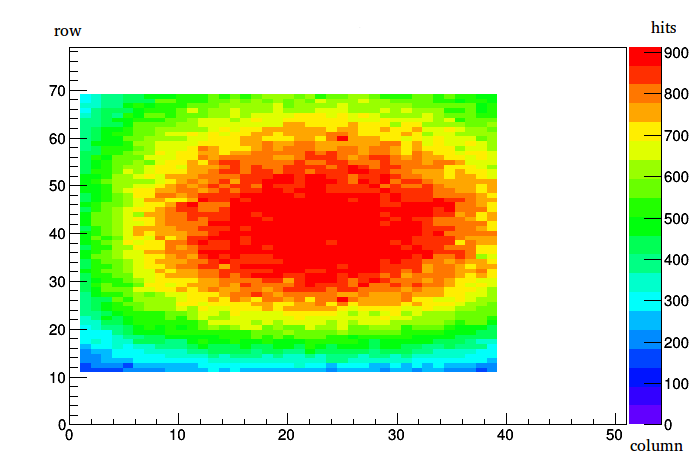
\includegraphics[width=0.47\textwidth]{hitmap1}\label{phitmap1}}
	\hfill
	\subbottom[Analogue plane 2 , partly masked]{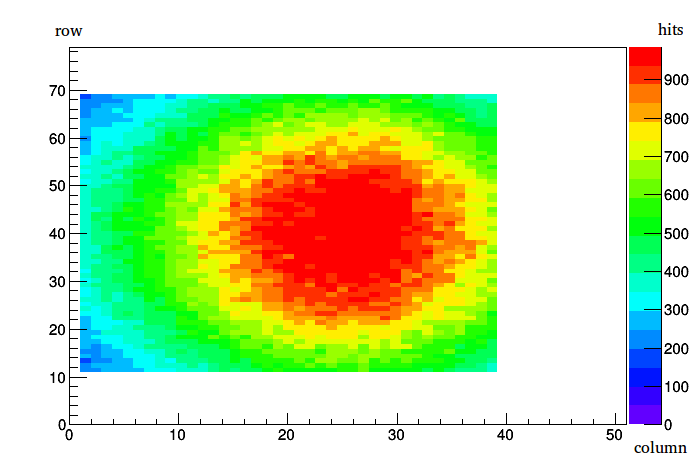
\includegraphics[width=0.47\textwidth]{hitmap2}\label{phitmap2}}
	\caption{Hitmaps of run $313$}
	\label{phitmap}
\end{figure}\no
% ========================================================
\subsection{Alignment}
A particle crossing the telescope generates hits within the telescope, with that information one tries to reconstruct the track of the passing particle. In order to reconstruct the track as good as possible the positions of each plane relative to each other must be known as good as possible. In reality the planes are not aligned perfectly due to indifferent mountings or even badly aligned if different types of planes are used together. In the alignment one uses multiple tracks of particles to find the spatial offsets in $x$ and $y$ and the rotation angle in phi of each plane.\\
First of all, special events have to be selected that can be used for tracking, because tracking gets more accurate the more points are used. In order to select those events, the hits of every event are grouped together to clusters. If the particle creates a lot electrons in the sensor or the sensor is hit close to the border between pixels, the charge can be shared between a couple of pixels. Therefore hits in consecutive pixels are put into a cluster whose centre is weighted by the amount of charge in each pixel. Only events with exactly one cluster in each plane are selected for the alignment.\\
The $z$ position of each plane is precisely measured with a solid gauge and is fixed, since the precision of the alignment in $z$ direction is not that good. Looping over all tracks and employing an iterative algorithm that uses the plane closest to beam as reference, the other planes are first rotated around the $z$-axis and then translated in $x$ and $y$ direction until the residuals of the tracks are minimal. In order to do that, it needs the relative $z-$position of the planes as input. The rotation angle and the two translations are then saved for every plane and can be used in the following. 
% ========================================================
\subsection{Tracking}
In a first step all hits are aligned using the rotation angle and the translations from above. Also for the tracking only events are used that have a single cluster in each plane. Then the points of the cluster centres are fitted using linear regression with errors that are rated with the digital resolution of $1/\sqrt{12}\,$pixelsize. It is possible to use the extracted residuals to get a better estimate for the errors, s.t. they can be adjusted for each pane separately.\\
Using the informations of the fit, the slope of the $x-$ and $y-$projections of the tracks is filled into a histograms, which are then fitted by a Gaussian to measure the centre. Examples of these histograms are illustrated in \ar{pslope}. If the slope distribution is not centred around the zero the planes are not perpendicular to the beam. That is why this information can be used to physically align the telescope to the beam. Furthermore the $\upchi^{2}$ for both projections as well as for the track are filled into histograms as well. The $\upchi^{2}$ is good indicator for the quality of the tracks and can be used as selection criterion for further analysis. Examples of these histograms are shown in \ar{pchi}.
The software will also plot an event display for selected events of every run that shows the path of the track and hits in each plane, as well as a 3D illustration of the track. This is depicted in \ar{pevent} and \ar{p3D}.\\
In order to check the alignment the distributions of the residuals for each plane is drawn. Examples are shown in \ar{pres}.
\begin{figure}[ht]
	\centering
	\subbottom[Slope of the $x$-projection.]{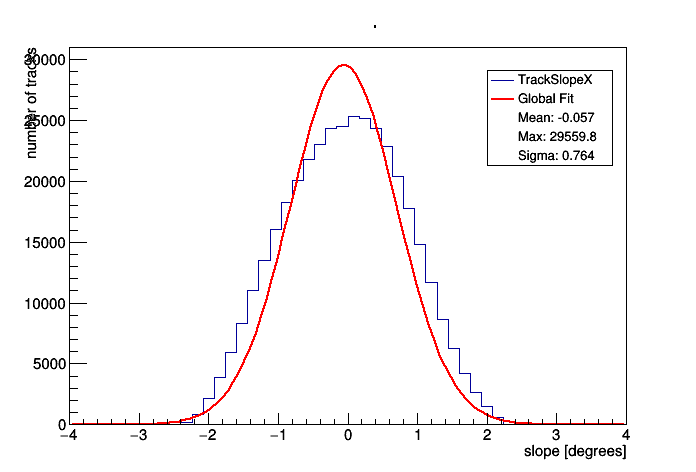
\includegraphics[width=0.47\textwidth]{tracking/slopex}\label{pslope1}}
	\hfill
	\subbottom[Slope of the $y$-projection]{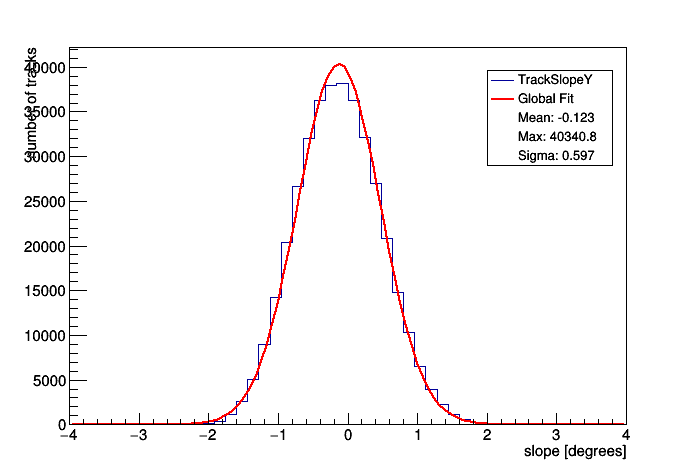
\includegraphics[width=0.47\textwidth]{tracking/slopey}\label{pslope2}}
	\caption{Track slopes of run $313$.}
	\label{pslope}
\end{figure}\no
\begin{figure}[ht]
	\centering
	\subbottom[$\upchi^{2}$]{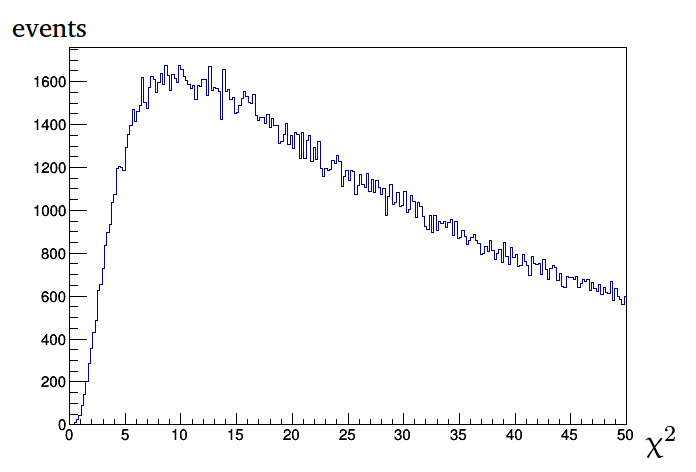
\includegraphics[width=0.31\textwidth]{tracking/chi}\label{pchia}}
	\hfill
	\subbottom[$\upchi^{2}$ of the $y$-projection]{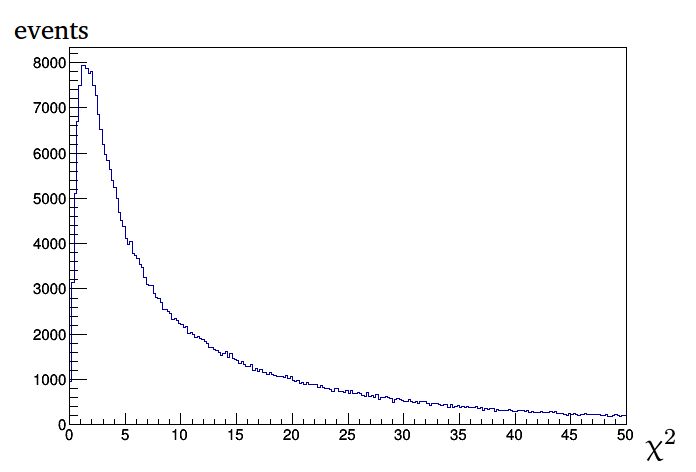
\includegraphics[width=0.31\textwidth]{tracking/chix}\label{pchi1}}
	\hfill
	\subbottom[$\upchi^{2}$ of the $y$-projection]{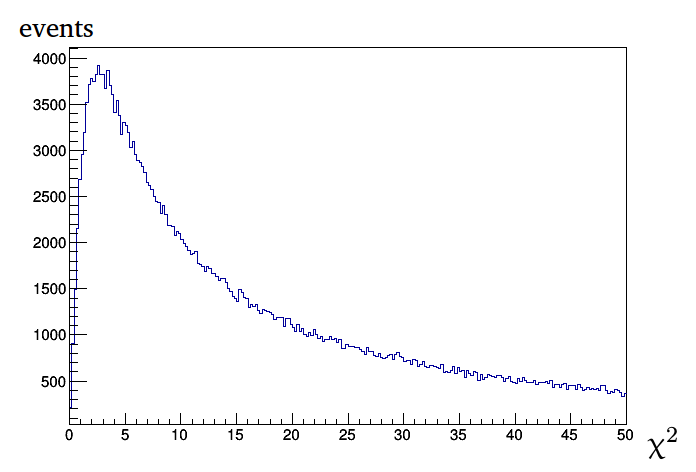
\includegraphics[width=0.31\textwidth]{tracking/chiy}\label{pchi2}}
	\caption{$\upchi^{2}$s of run $313$.}
	\label{pchi}
\end{figure}\no
\begin{figure}[ht]
	\centering
	\subbottom[Residual in $x$.]{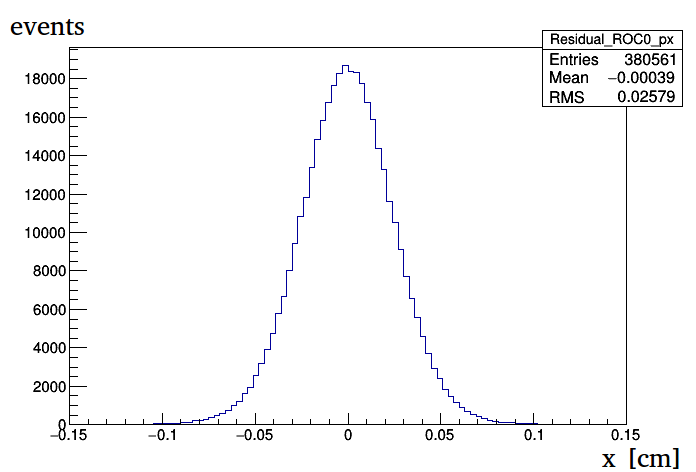
\includegraphics[width=0.47\textwidth]{tracking/resx}\label{pres1}}
	\hfill
	\subbottom[Residual in $y$.]{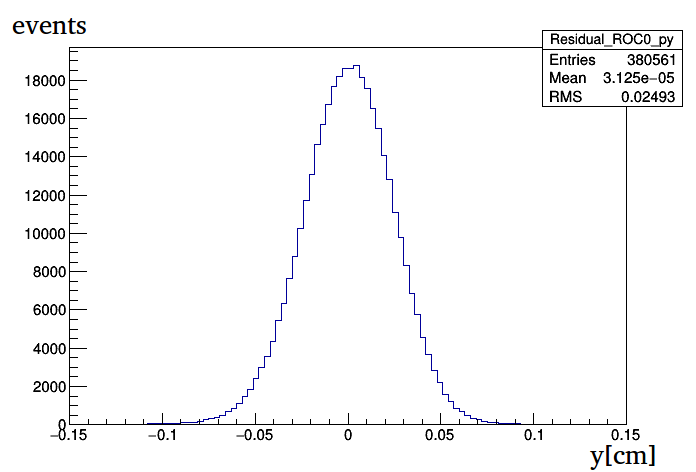
\includegraphics[width=0.47\textwidth]{tracking/resy}\label{pres2}}
	\caption{Residual of plane $0$ of run $313$.}
	\label{pres}
\end{figure}\no
\begin{figure}[ht]
	\centering
	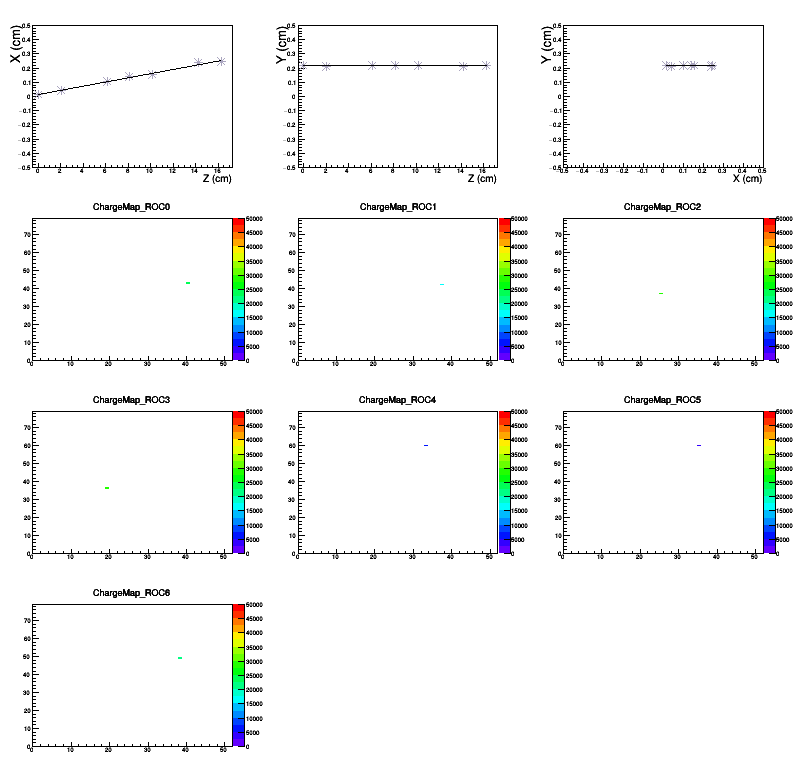
\includegraphics[width=0.95\textwidth]{tracking/event}
	\caption{Event display for an event of run $313$ including the fit}
	\label{pevent}
\end{figure}\no
\begin{figure}[ht]
	\centering
	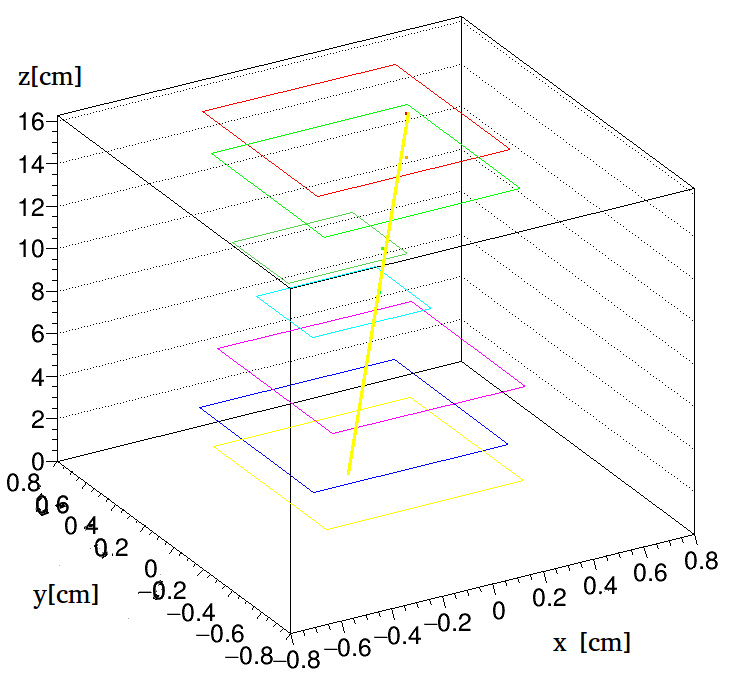
\includegraphics[width=0.5\textwidth]{tracking/3D}
	\caption{3D track display for an event of run $313$ including the fit}
	\label{p3D}
\end{figure}\no
% ========================================================
% PULSE HEIGHTS
% ========================================================
\subsection{Pulse Heights}
The pulse height provides information of the energy the particle has left inside the sensor. In order to convert the \ac{ADC} values of the data into electrons, the results of the pulse height calibration in \ar{spulseheight} are used. With the help of them the charge of each cluster can be achieved by summing up all charges of its consisting hits. Then The charge of the clusters with one, two ore three and more hits are compared with the distribution of all cluster sizes. Examples for a digital and an analogue chip are shown in \ar{pphmap1} and \ar{pphmap2}\\
For both digital and analogue distributions single hits are dominant and for the digital one the peak of each sub distribution is roughly at the same spot, which is expected. For the analogue though, the distributions of the bigger clusters is shifted to lower energies, which is not yet understood and has to be analysed further. The peaks of the main distributions of digital and analogue \ac{ROC} are roughly at the same energy of $25000$ electrons. Alltogether, the \ac{PH} calibration is working well for the digital chip.\\
As demonstrated in \ar{plandaufit} the signal of the digital chip is nicely landau shaped, as would be expected by theory.\\
By looking at the longer range of the energy in \ar{plong1log} and \ar{plong6log} a second prominent peak shows up at around $120000$ and $170000$ electrons for analogue and digital \ac{ROC} respectively. The \ac{PSI} pion beam consists also a tiny fraction of protons. Since protons are about seven times heavier than pions and the particles are with a momentum of $260\,$MeV/c still in the $1/\beta$ range of the Bethe-formula \ar{ebethe} the proton should lose of the order of $10$ more energy than a pion. Due to that, the second peak should belong to protons and the first one to pions. By looking at the size of the proton peaks one can also see that the total number of protons for the digital chip is an order of ten times smaller then for the analogue \ac{ROC}. In the set-up of the picture the analogue plane was closer to the beam with other planes in between the two. That is why the lower number of protons is expected as they have a higher stopping power, which also means that the protons are more likely to scatter. 
\newpage
\begin{figure}[ht]
	\centering
	\subbottom[analogue \ac{ROC} short scale]{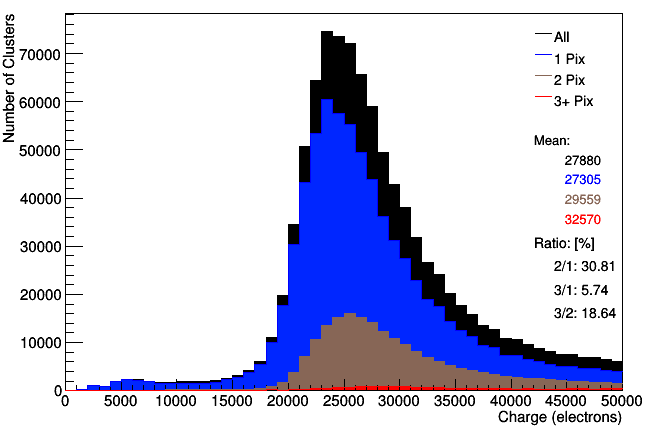
\includegraphics[width=0.47\textwidth]{tracking/ph6}\label{pph6}}
	\hfill
	\subbottom[digital \ac{ROC} short scale]{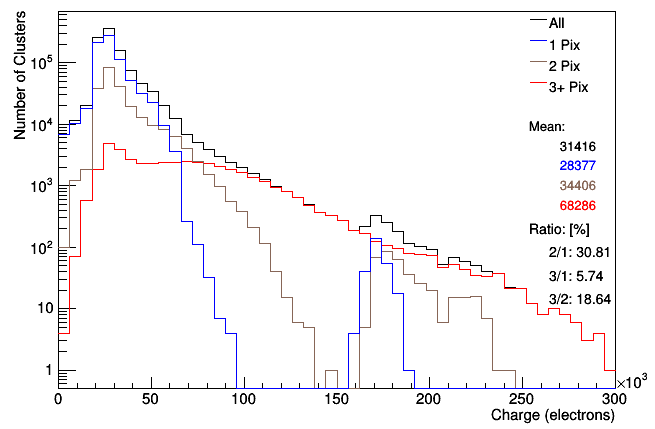
\includegraphics[width=0.47\textwidth]{tracking/long6log}\label{plong6log}}
	\caption{Pulse height distributions for a digital plane}
	\label{pphmap1}
\end{figure}\no
\begin{figure}[ht]
	\centering
	\subbottom[analogue \ac{ROC} long scale, logarithmic y-axis]{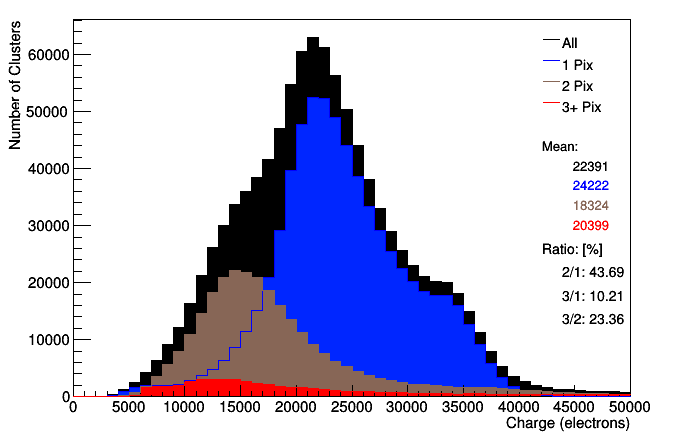
\includegraphics[width=0.47\textwidth]{tracking/ph1}\label{pph1}}
	\hfill
	\subbottom[digital \ac{ROC} long scale, logarithmic y-axis]{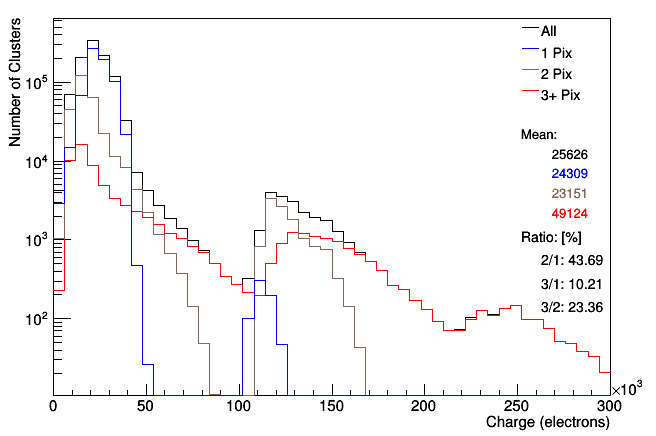
\includegraphics[width=0.47\textwidth]{tracking/long1log}\label{plong1log}}
	\caption{Pulse height distributions for an analogue plane}
	\label{pphmap2}
\end{figure}\no
\begin{figure}[ht]
	\centering
	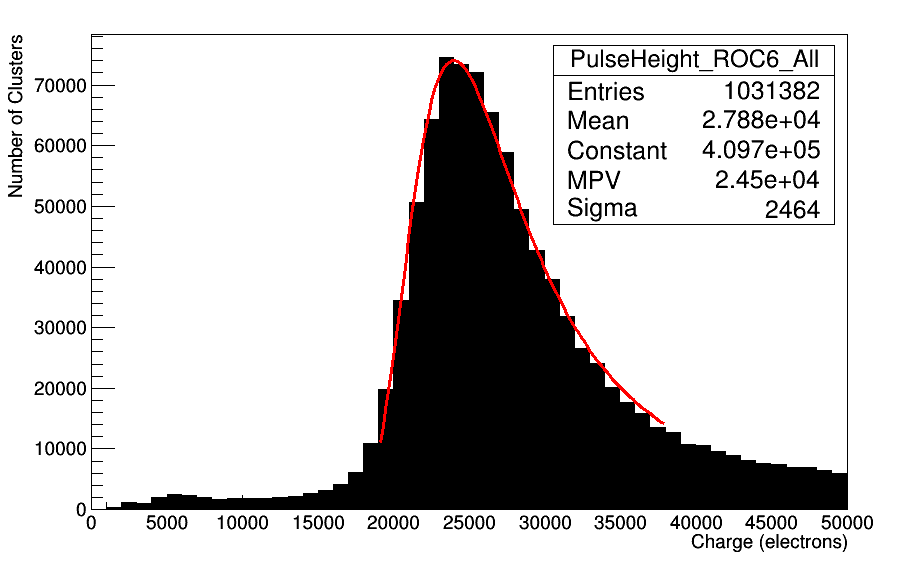
\includegraphics[width=0.65\textwidth]{tracking/landaufit}
	\caption{Landau fit of the cluster charge distribution of a digital \ac{ROC}}
	\label{plandaufit}
\end{figure}\no
% RESOLUTION
% ========================================================
% \section{Resolution}
% % ========================================================
% % DELTA RAYS
% % ========================================================
% \section{Delta Rays}
% % ========================================================
% % KEITHLEY CURRENTS
% % ========================================================
% \section{Keithley Currents}
% % ========================================================
% % LOG READER
% % ========================================================
% \section{EUDAQ Log Reader}
% ========================================================
% TO GET IT COMPILED
% ========================================================
\chapter*{List of Acronyms}
\begin{acronym}[Bash]
	\acro{PUC}{pixel unit cell}
	\acro{ROC}{readout chip}
	\acro{TBM}{token bit manager}
	\acro{UB}{ultra black}
	\acro{B}{black}
	\acro{CMS}{Compact Muon Solenoid}
	\acro{LHC}{Large Hadron Collider}
	\acro{CERN}{European Organization for Nuclear Research}
	\acro{DAC}{digital to analogue converter}
	\acro{ADC}{analogue to digital converter}
	\acro{LD}{last DAC}
	\acro{DTB}{digital test board}
	\acro{ATB}{analogue test board}
	\acro{ETH}{Eidgen{\"o}ssische Technische Hochschule}
	\acro{FPGA}{Field Programmable Gate Array}
	\acro{PSI}{Paul Scherrer Institut}
	\acro{HV}{high voltage}
	\acro{TTL}{Transistor-Transistor-Logic}
	\acro{PLL}{phase-locked loop}
	\acro{FIFO}{First In - First Out}
	\acro{HAL}{hardware abstraction layer}
	\acro{API}{application programming interface}
	\acro{GUI}{graphical user interface}
	\acro{CLI}{command line interface}
	\acro{DAQ}{data acquisition}
	\acro{CPU}{central processing unit}
	\acro{PG}{pattern generator}
	\acro{I2C}[I$^{2}$C]{Inter-Integrated Circuit}
	\acro{DUT}{device under test}
	\acro{TCP}{Transmission Control Protocol}
	\acro{TU}{trigger unit}
	\acro{COM}{centre of mass}
	\acro{PSB}{Proton Synchrotron Booster}
	\acro{PS}{Proton Synchrotron}
	\acro{SPS}{Super Proton Synchrotron}
	\acro{ALICE}{A Large Ion Collider Experiment}
	\acro{ATLAS}{A Toroidal LHC Apparatus}
	\acro{LHCb}{Large Hadron Collider beauty}
	\acro{LHCf}{ Large Hadron Collider forward}
	\acro{TOTEM}{TOTal Elastic and diffractive cross section Measurement}
	\acro{SUSY}{supersymmetry}
	\acro{HCAL}{hadronic calorimeter}
	\acro{ECAL}{electromagnetic calorimeter}
	\acro{CTR}{calibrate trigger reset}
	\acro{MIP}{minimum ionising particle}
	\acro{PM}{photo multiplier}
	\acro{TLU}{trigger logic unit}
	\acro{PH}{pulse height}
	\acro{DC}{double column}
	\acro{DESY}{Deutsches Elektronen-Synchrotron}
	\acro{RAM}{Random-Access Memory}
	\acro{PCB}{printed circuit board}
	\acro{PLT}{Photo Luminosity Telescope}
	\acro{RPC}{remote procedure calls}
\end{acronym}
\bibliographystyle{plain}
% \bibliography{refs}
\end{document}
